%! TEX root = main.tex  %
\documentclass[main.tex]{subfiles} % Wichtig!

\begin{document}


\subsection{Projektmanagement}

Wie im vorhergehenden Kapitel «Agile Entwicklung - Automatisiertes Testen / DevOps»
beschrieben, sind sämtliche gesammelten Informationen und gefällten Entscheidungen
in einem Artefakt zu vermerken. Anleitungen für typische Softwareartefakte können
dabei nützliche Wegleitungen sein.

\subsection{Grobplanung}
Die Grobplanung zeigt die wichtigsten Meilensteine des Projekts auf. Zudem werden
die wichtigsten Aufgaben und deren zeitliche Abfolge dargestellt.

\begin{figure}[h]
    \hspace{-0.075\linewidth} % 15% divided by 2 to center the image
    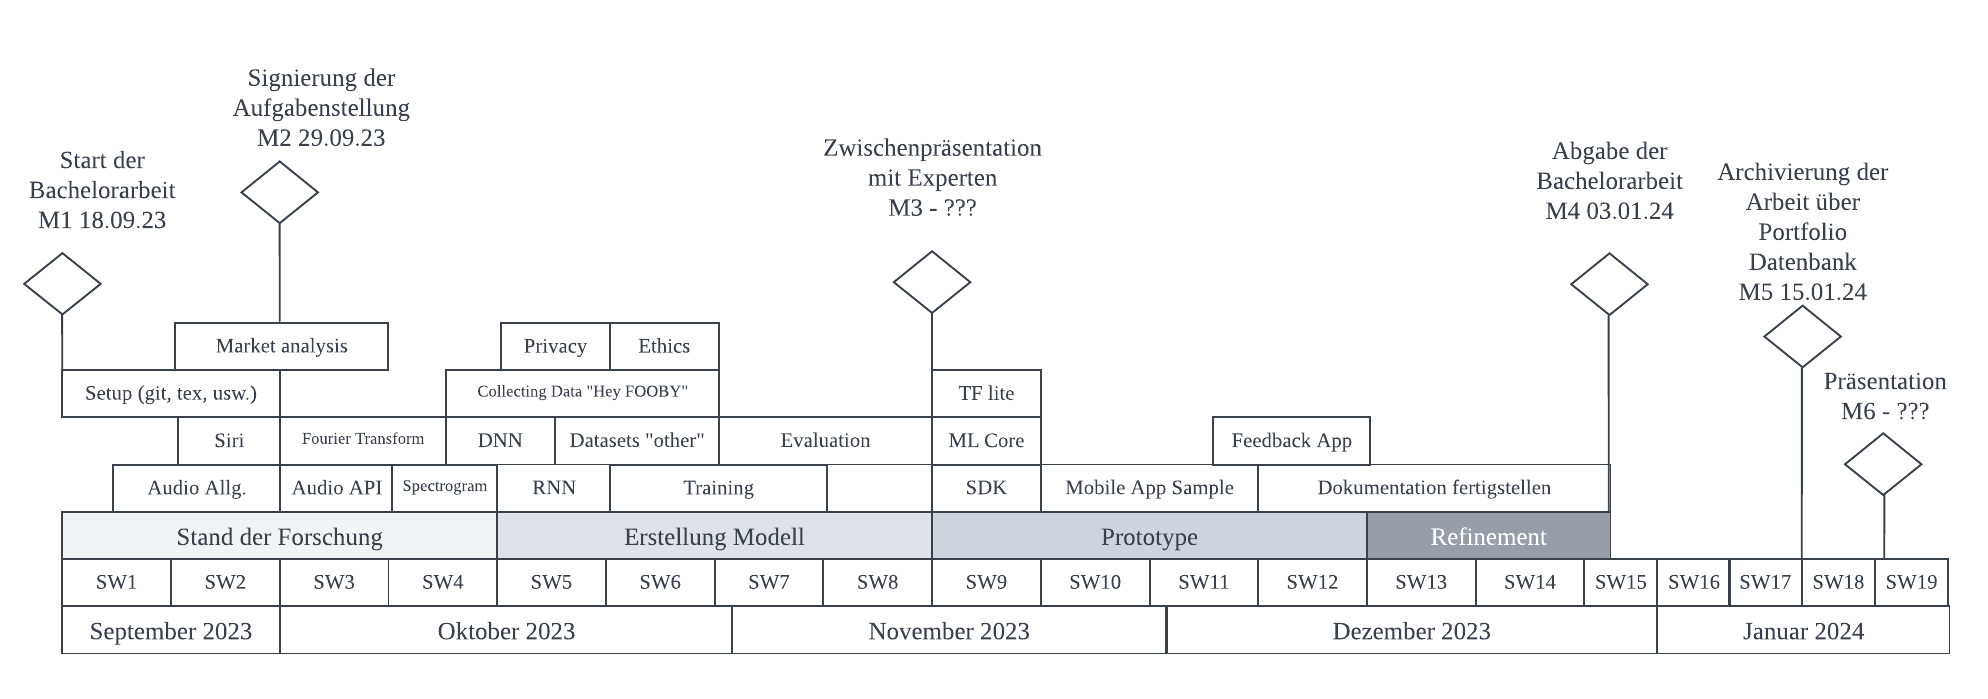
\includegraphics[width=1.15\linewidth]{img/projectplan.png}
    \caption{Grobplanung}
    \label{fig:grobplanung}
\end{figure}




\subsubsection{Produkt Backlog}

In der Vorbereitungsphase kann ein anfängliches Produkt Backlog als einfache Tabelle
dargestellt werden. Ein Beispiel für eine solche Tabelle ist in Abbildung 5 dargestellt.



\begin{figure}[h]
    \centering
    
\includegraphics[width=0.7\linewidth]{img/placeholder.png}
    \caption{Tabelle für das anfängliche Product Backlog}
    \label{fig:backlog_table}
\end{figure}


\subsubsection{Risikomanagement}
Risikomanagement dient dem Zweck, mögliche Probleme vorwegzunehmen. Die Verwendung von
Checklisten, Brainstorming mit den Anspruchsgruppen und die von Erfahrungen
aus früheren Projekten sind mögliche Strategien zur Identifikation möglicher Risiken.

\begin{table}[h]
    \centering
    \caption{Beispiel-Tabelle für Risikomanagement}
    \begin{tabular}{|c|c|c|}
        \hline
        Kopf 1 & Kopf 2 & Kopf 3 \\
        \hline
        Wert 1 & Wert 2 & Wert 3 \\
        \hline
        Wert 4 & Wert 5 & Wert 6 \\
        \hline
    \end{tabular}
    \caption{Eine einfache Tabelle}
    \label{tab:meineTabelle}

\end{table}



\end{document}

